% !TEX root = ./informe.tex
\section{Experimentación general}

Dado que nuestros análisis estaban enfocados en los peores casos, es momento de considerar cómo son nuestras soluciones si consideramos casos promedios.  \\

Consideramos que un grafo de $n$ nodos es promedio cuando generamos sus aristas al azar. Esto significa que las conexiones entre nodos será aleatoria, pero que la cantidad de aristas estará predeterminada con algun porcentaje, para poder separar mejor los diferentes casos de análisis. En particular, mostraremos los casos donde hay 50\% y 75\% de aristas. Demás porcentajes resultaron muy poco interesantes por tener muy pocas aristas o demasiadas. Como última aclaración, para todas las instancias de búsqueda local, la cantidad de repeticiones usadas es $2000$, a menos que se mencione explícitamente. \\

Nuestra intención es comparar exactamente qué tan mejores o peores son los diferentes algoritmos utilizados. Para esto, para cada tamaño de $n$ generamos un grafo al azar (con cierto porcentaje de aristas) y comparamos las soluciones obtenidas por todas las técnicas. Lo que sigue no son promedios, sino las soluciones finales para algun algoritmo aleatorio dado \todo{¿no es `para algún \textbf{caso} aleatorio dado'?}. \\

{\centering
    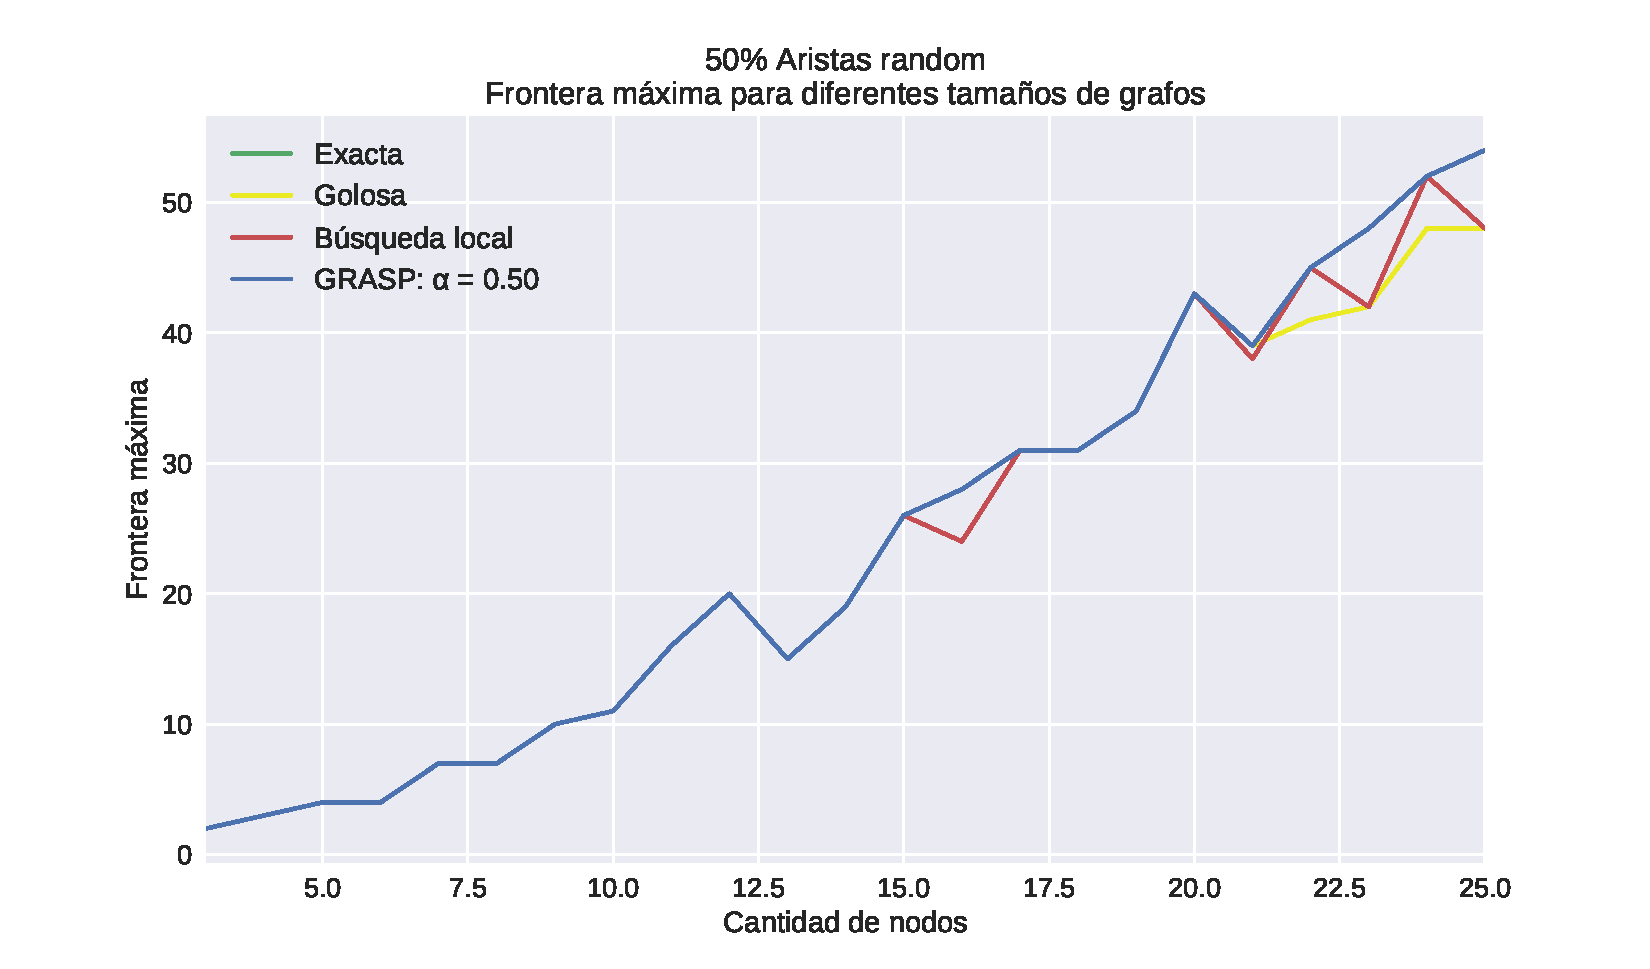
\includegraphics[width=0.9\textwidth]{informe/imgs/exp_random50_frontera_todos_v2.pdf}
    \captionof{figure}{$\uparrow$ Exacta y GRASP comparten la misma curva}
}
$ $ \newline

Los resultados son los que nuestros análisis anteriores apuntaban. Debemos tener en cuenta que son valores de $n$ pequeños (para poder comparar con el algoritmo exacto), veremos más adelante comparaciones para $n$ mayores. \\

Observamos que GRASP es la mejor técnica de las presentadas para resolver el problema. De hecho, comparte la misma curva que el algoritmo exacto. Le siguen el algoritmo de búsqueda local, y por último el goloso. Como sospechábamos, si bien en el análisis para un ``grafo malo'' el greedy era extremadamente malo, aquí podemos notar que para grafos en general conseguimos una aproximación bastante buena. \\

Analicemos tambíen que pasa con los tiempos de cómputo. Como era esperable, el tiempo del algoritmo exacto crece muy rápidamente, así que mostramos el gráfico en \textit{escala logarítmica}. En general son tiempos esperados, pero es interesante notar que GRASP tiene una constante asociada mucho mas elevada que los demás. \\

{\centering
    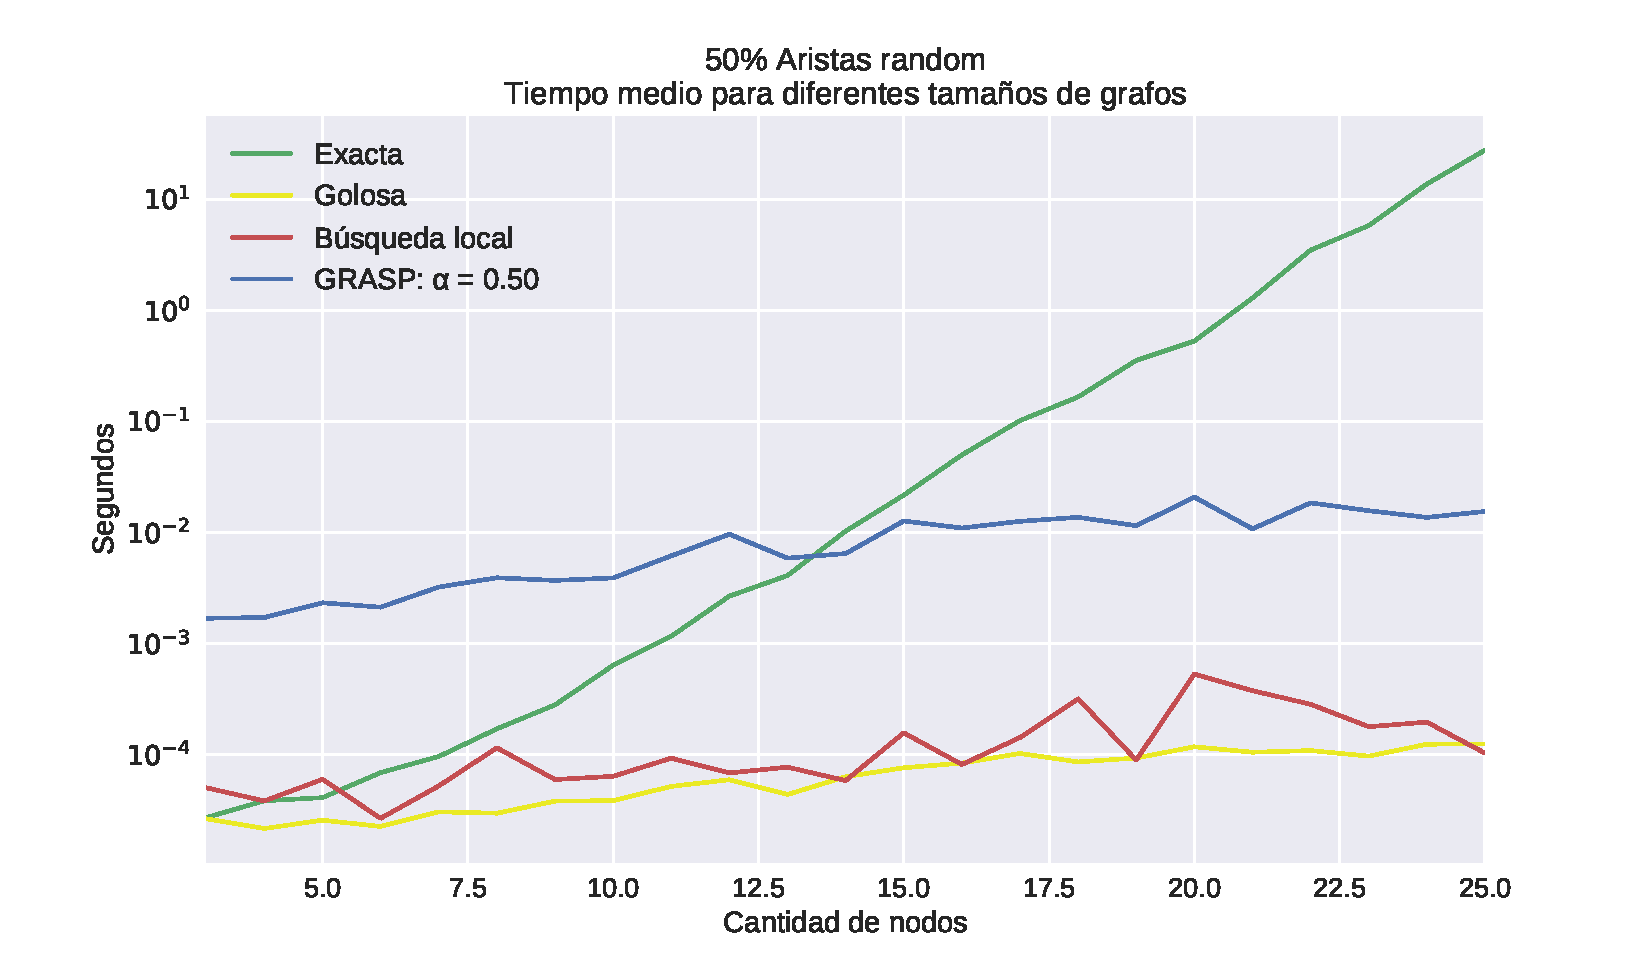
\includegraphics[width=0.9\textwidth]{informe/imgs/exp_random50_tiempo_todos_v2.pdf}
    \captionof{figure}{$\uparrow$ Escala logarítmica}
}
$ $ \newline

Repetimos el experimento pero para grafos con 75\% de aristas. Sin embargo, todos los algoritmos nos dan la misma solución (¡La óptima!). Esto tiene que ver con la densidad del grafo, y probablemente porque estamos viendo tamaños pequeños. \\

{\centering
    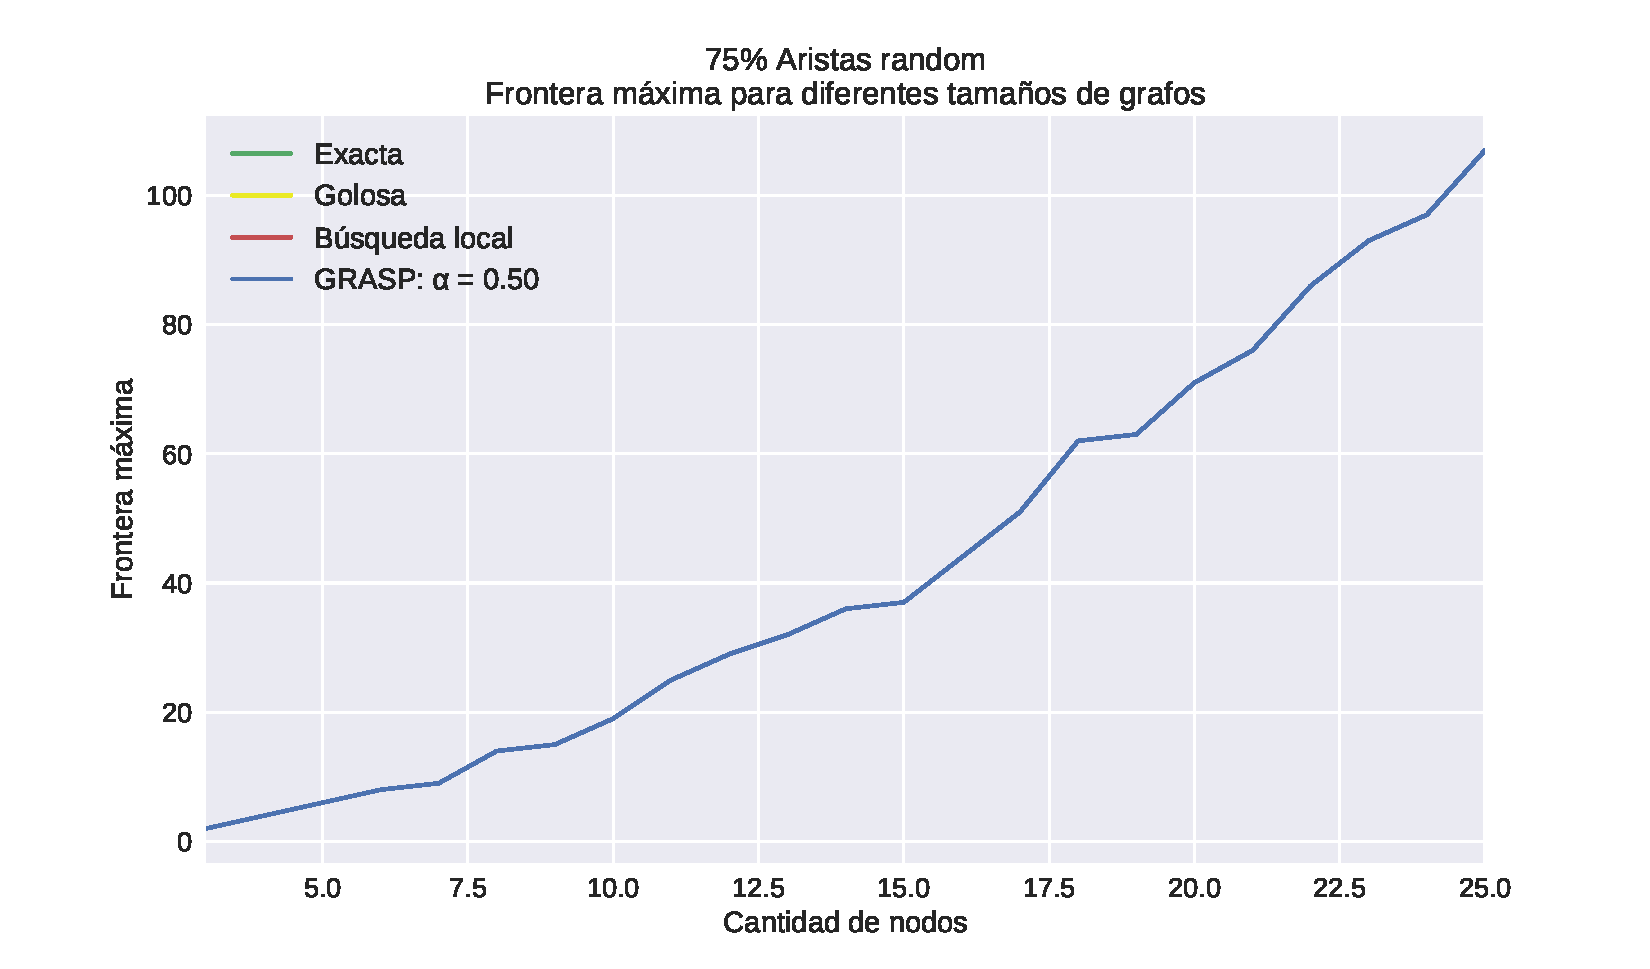
\includegraphics[width=0.9\textwidth]{informe/imgs/exp_random75_frontera_todos_v2.pdf}

}
$ $ \newline

Veamos que sucede si hacemos crecer $n$. Dado que no podemos realizar las pruebas para el algoritmo exacto debido a su complejidad temporal, no lo incluimos en el gráfico. No tenemos ninguna certeza de cuán cerca o lejos están de la solución óptima, pero es interesante observar como varían las diferentes soluciones. No incluímos 75\% aristas pues es idéntico al de 50\%. \\

{\centering
    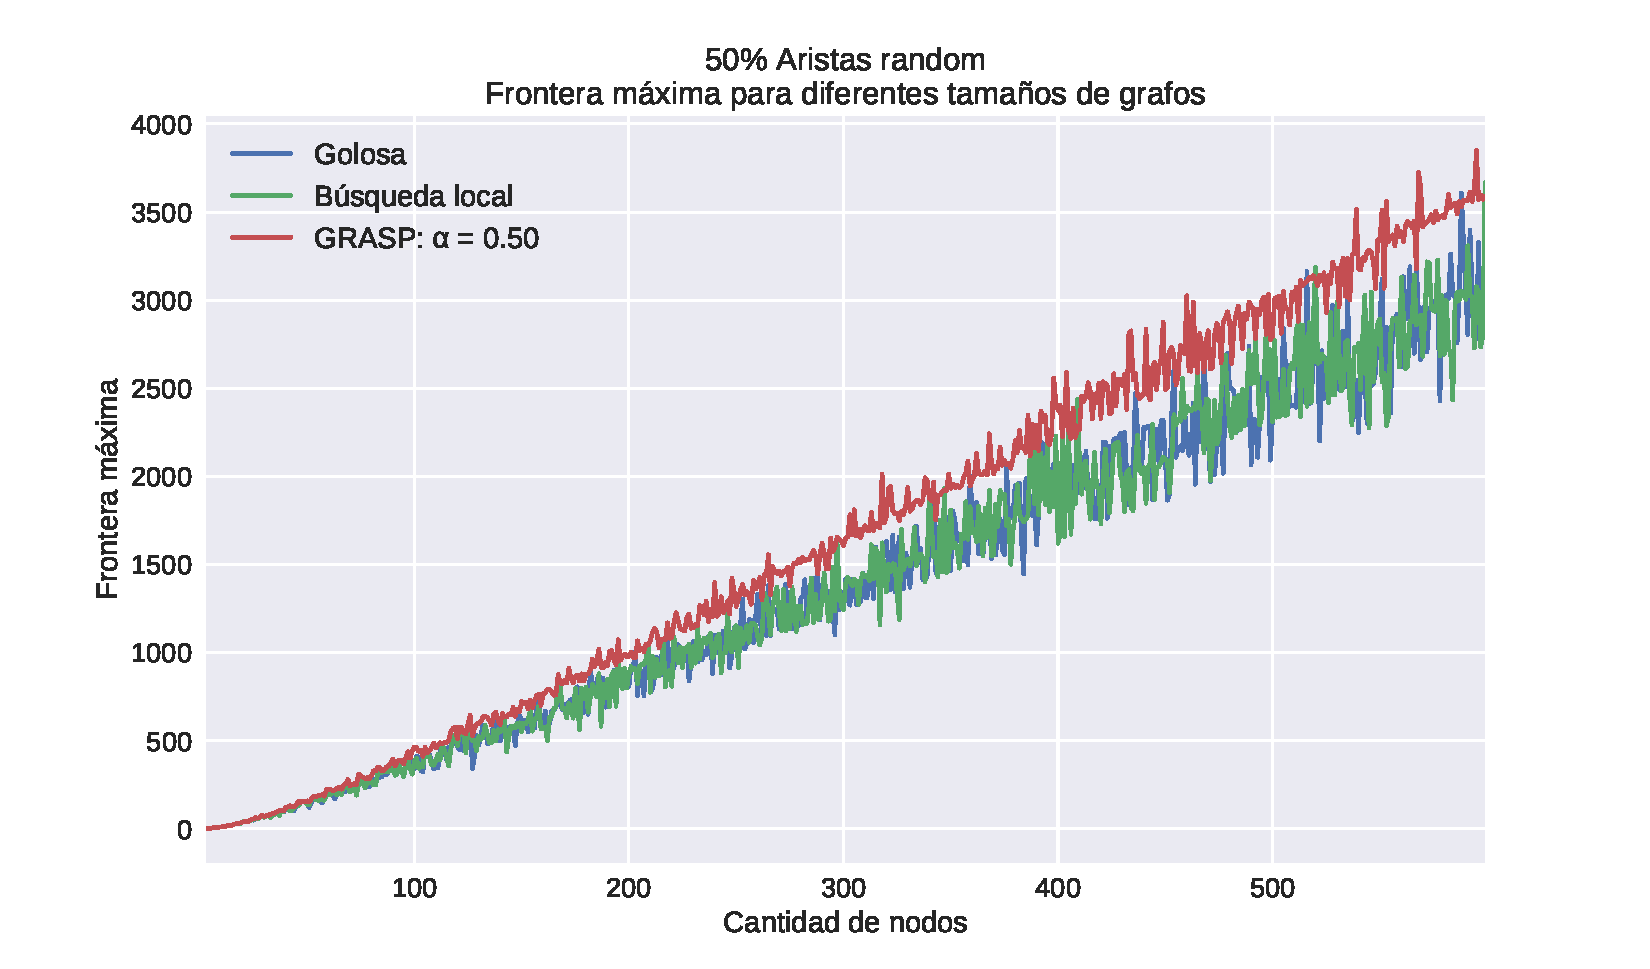
\includegraphics[width=0.9\textwidth]{informe/imgs/exp_random50_frontera_todos_ngrande.pdf}

}
$ $ \newline

Como esperábamos, GRASP es la mejor alternativa que tenemos para resolver el problema de CMF. El componente random sumado a la cantidad de repeticiones hacen que sea superior a los demás algoritmos, en términos de aproximación a la solución óptima. Variando la cantidad de $repsGrasp$ no obtuvimos diferencias significativas. En el gráfico se muestra con $repsGrasp = 50$. \\

GRASP es mejor, ¿pero a qué costo? Mostramos el gráfico en \textit{escala logárítmica} debido al tamaño de los tiempos de GRASP en comparación a los demás. Podemos observar claramente que el costo temporal es incluso mayor al esperado, dónde para $n = 600$ se demora aproximadamente 3 segundos. Esto entra en linea con la constante que habiamos observado en el anterior gráfico de tiempos. Es más que razonable, ya que estamos repitiendo dos algoritmos $O(n^5)$ en este caso $50$ veces. \\

{\centering
    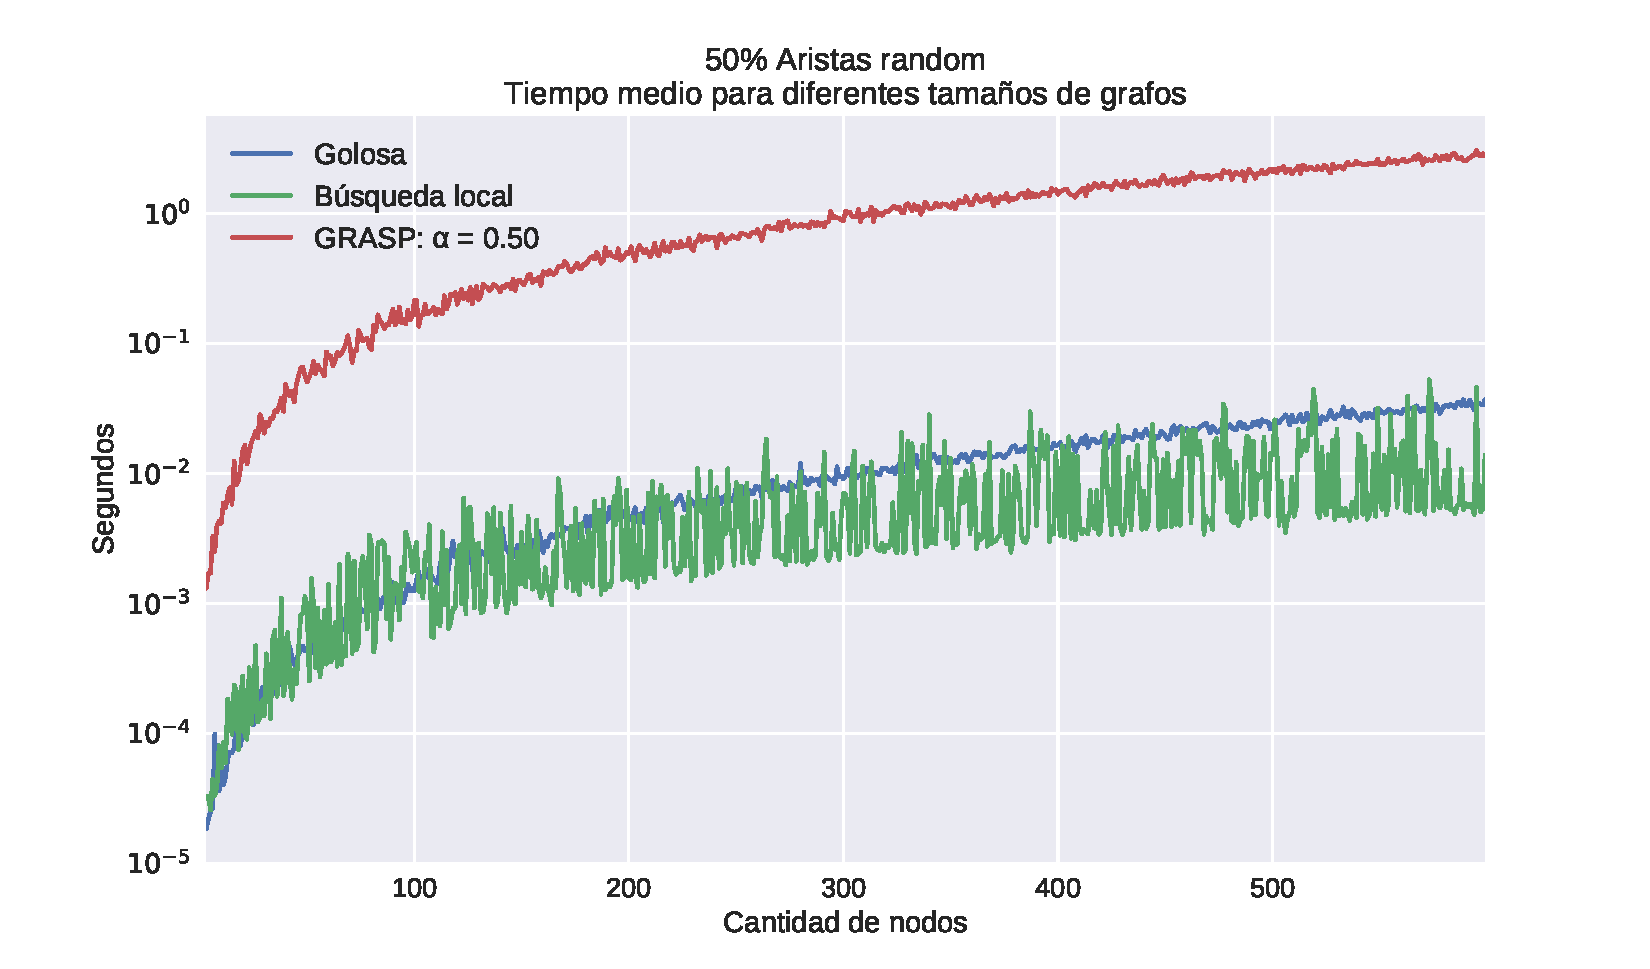
\includegraphics[width=0.9\textwidth]{informe/imgs/exp_random50_tiempo_todos_ngrande_logy.pdf}

}
$ $ \newline

El caso de tiempos de 75\% aristas no lo mostramos por ser idéntico en forma al anterior, pero en ese caso, con $n = 600$, GRASP tarda aproximadamente 17 segundos. Pueden disminuirse la cantidad de iteraciones para obtener una mayor eficiencia en términos del tiempo, pero a medida que $n$ crece GRASP es el primero que se vuelve inutilizable.

% No vale la pena por ser igual a 50%
% {\centering
%     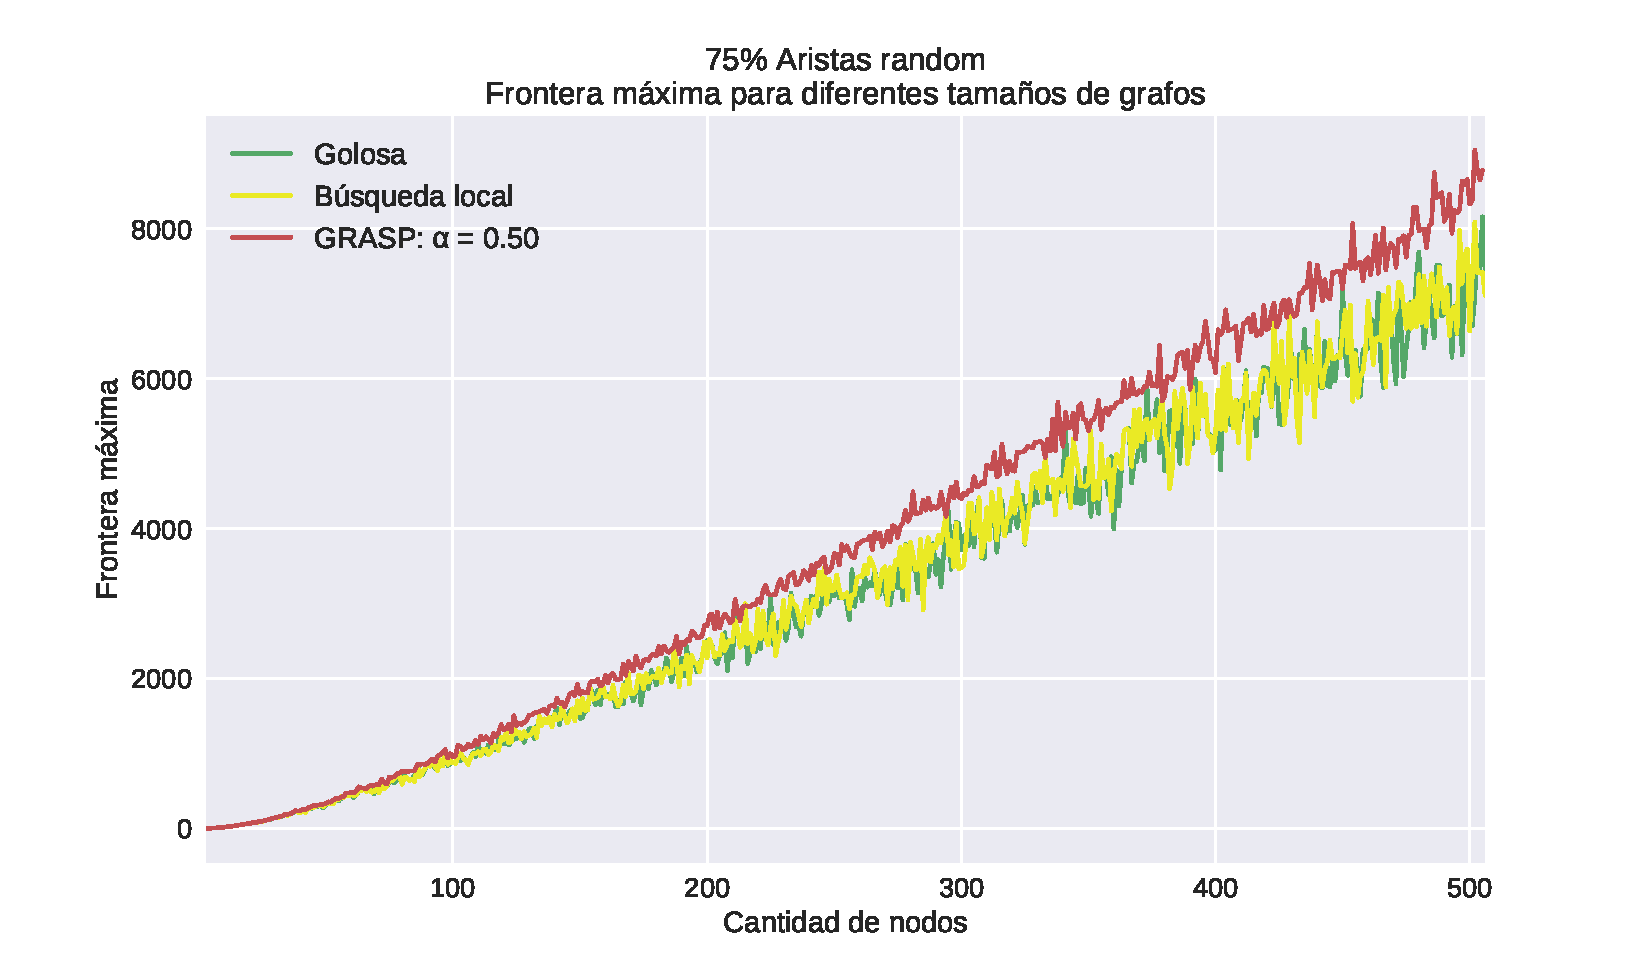
\includegraphics[width=1\textwidth]{informe/imgs/exp_random75_frontera_todos_ngrande.pdf}
% }


\subsection{Conclusión}

El objetivo de este trabajo era la investigación de diferentes técnicas para resolver el problema de Clique de Máxima Frontera. Sabemos que no se conoce hasta el momento ningún algoritmo exacto que lo resuelva en tiempo polinomial, por lo que mostramos una única forma de resolverlo de forma exacta, con complejidad temporal exponencial. \\

Vimos que el algoritmo exacto es inutilizable en la práctica para grafos con mas de 30 nodos, así que en la práctica es necesario recurrir a heurísticas que resuelvan el problema. \\

Consideramos un algoritmo sencillo, \textbf{greedy}, para intentar conseguir una buena solución. Lo que logramos encontrar fue un algoritmo exponencialmente mas rápido que en general da aproximaciones razonables. Encontramos además, al menos un tipo particular de grafos, los ``grafos malos'', para los cuales demostramos que la diferencia entre la solución óptima y la solución greedy tendía a infinito. \\

Intentando ahora poder solucionar el problema de ``grafos malos'', consideramos una heurística de \textbf{búsqueda local} para mejorar soluciones preexistentes, en dónde analizamos distintas formas de movernos a soluciones similares. Si bien en ocasiones logramos mejorar el método anterior, seguimos cayendo en el problema de que una vez llegados a un extremo local ya nos era imposible salir de ahí pues ninguna solución en su vecindad la mejoraría. \\

Para finalizar, nos basamos en el paper citado \cite{paper_grasp} para construir una solución que use el método GRASP. Con la introducción de variables aleatorias en conjunto con cierta estrategia golosa, logramos escapar del problema de los extremos locales pudiendo lograr así soluciones óptimas con gran probabilidad en nuestros grafos originales. \\

Una vez analizadas las distintas alternativas, probamos todos los algoritmos en una serie de grafos aleatorios, con diferentes porcentajes de aristas. Pudimos comprobar empíricamente lo analizado antes: GRASP produce los mejores resultados. Sin embargo, nos fue imposible dar una cota de distancia con respecto a la solución óptima porque no tenemos manera de conocer cuál es ésta solución sin poder correr el algoritmo exacto. \\